% !TeX root = ../main.tex
% Add the above to each chapter to make compiling the PDF easier in some editors.

\chapter{Evaluation}\label{chapter:evaluation}

We provide an evaluation of the performance of our model and compare it to other work.
Unless otherwise noted due to the nature of the evaluation, all results are evaluated on actual cardinalities.
Therefore, we detach our results from the ongoing issue of accurately estimating cardinalities~\parencite{leis2018job}.

\section{Generalization and Frequency Distribution}

\paragraph{Accuracy and Generalization across Databases.}
Figure~\ref{fig:database_q} shows the generalization capabilities of our model across different, unseen database instances.
This is ensured by training the model on all databases except the one being tested.

We see low p50 values across all databases and higher p90 and average values – we consider this a good accuracy performance.
The median Q-Error is below 1.5 for all databases and does not vary much across databases.
Although we find more variation in the average and p90 values, we conclude that the model is able to generalize across unseen database instances.
This finding applies to the queries of the ZeroShot training data we used.

Since we took the same data as the ZeroShot model, the median values indicate a comparable generalization performance to the ZeroShot model. 
Their median values across databases are in the same range~\parencite{zeroshot}.

\paragraph{Frequency Distribution.}
Figure~\ref{fig:qerror_freq} gives us a frequency distribution example of our model on the JOB-Benchmark
(we will use the JOB-Benchmark further in the evaluation).
Since the average and p90 values are higher than the p50 value across all databases, the distribution we observe is expected.

The majority of queries have a low Q-Error and only a few queries have a higher Q-Error.
With this skewed distribution we explain the higher average and p90 values.
\begin{figure}[htpb]
  \centering
  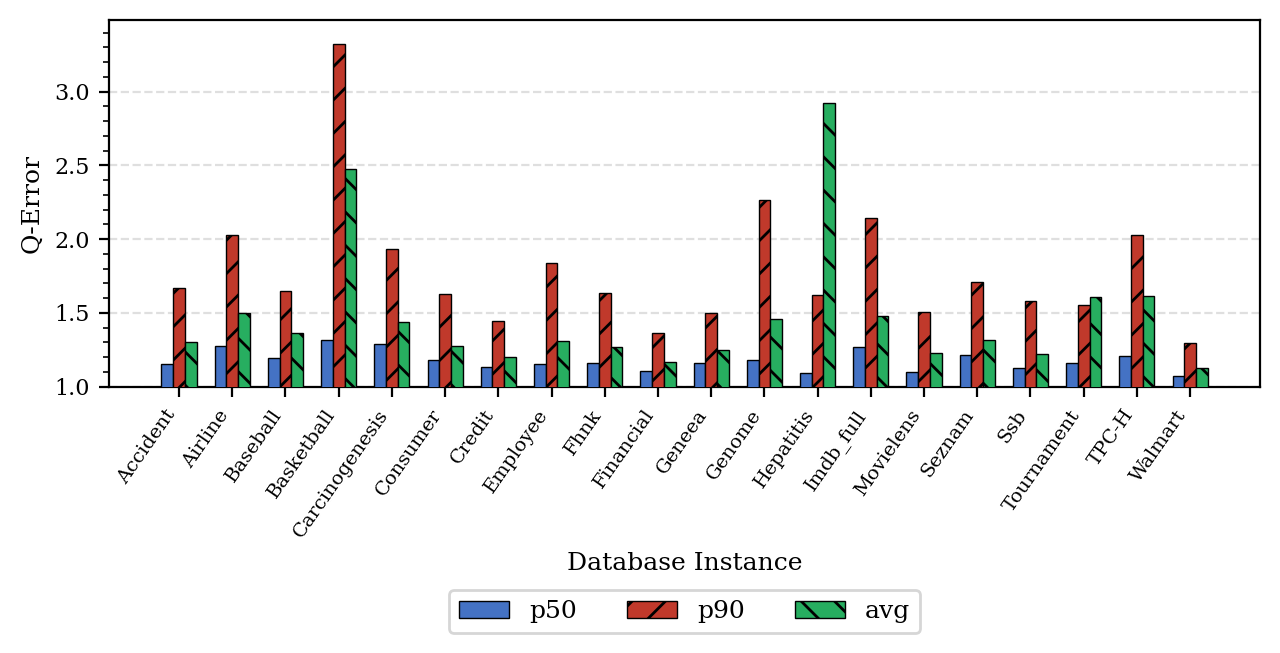
\includegraphics[width=\textwidth]{figures/database_q.png}
  \caption[Q-Error across Database Instances]{Q-Error (p50, p90, and average) of our model evaluated across all database instances. Each database is excluded from the training set when tested and plotted. All other databases are included in the training set. }\label{fig:database_q}
\end{figure}

\begin{figure}[htpb]
  \centering
  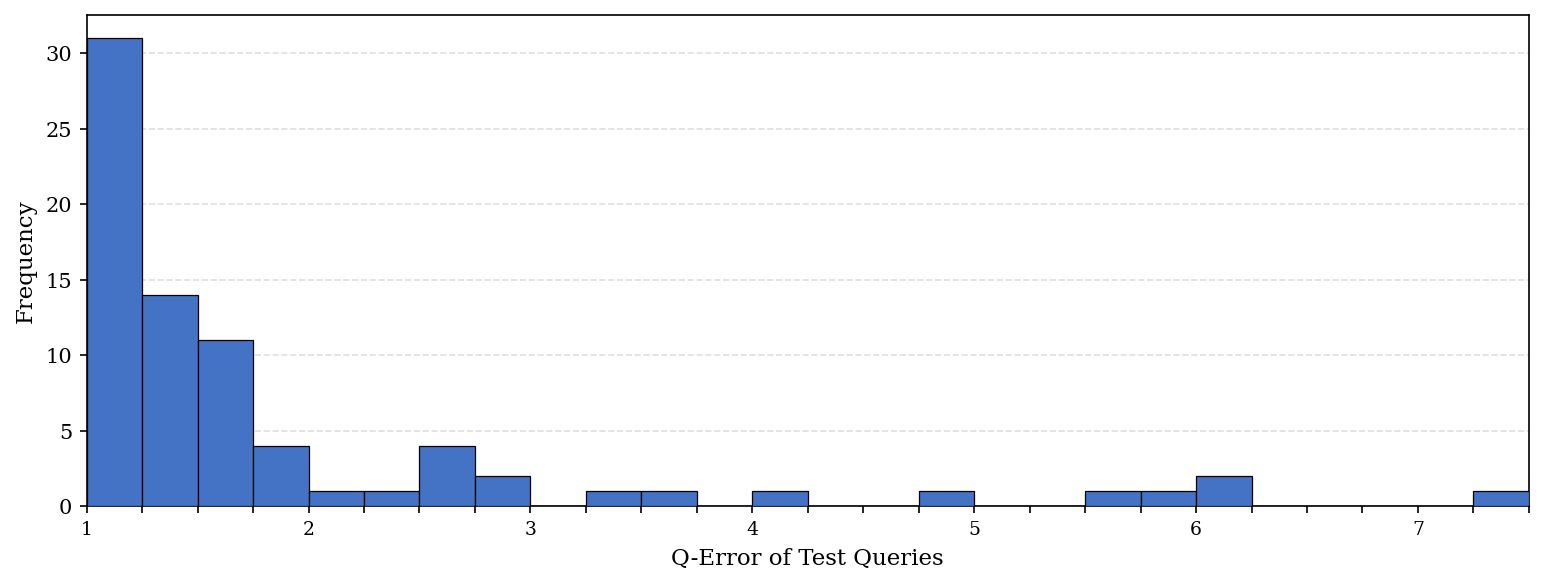
\includegraphics[width=\textwidth]{figures/qerror_freq.png}
  \caption[Q-Error Frequency Distribution]{Frequency distribution of Q-Error values across all available JOB queries.
  The model is trained on all databases except IMDB, which is the database of the JOB-Benchmark.}\label{fig:qerror_freq}
\end{figure}

\section{Comparison to Other Models}

\paragraph{Comparison to T3 (Umbra) and ZeroShot.}

The original T3 model for Umbra by Rieger and Neumann~\parencite{t3} and the ZeroShot model~\parencite{zeroshot} offer very good generalization performance across unseen databases.
Because T3 (Umbra) uses different queries for generalization testing, we cannot directly compare the generalization performance of our model to theirs.
However, Rieger \& Neumann compared both models on the JOB-Benchmark and reported excellent performance for both models~\parencite{t3}.

We also have JOB queries available for evaluation, so we can compare the models on that.
In the original comparison, Rieger \& Neumann compare the p50, p90, and average Q-Error values.
They had all 113 JOB queries available for evaluation. 

However, the provided ZeroShot training data came with data limitations.
Namely, longer-running queries are not included~\parencite{zeroshot}, so we only have 77 JOB queries available for evaluation.
As the number of total queries differ, it is not sensible to compare the p50 and p90 Q-Error values directly.
If the missing queries had a very high Q-Error, the p50 value of our model would be higher than now and comparing using the current p50 value would be misleading.
This also applies to the p90 value.

Considering how the median is calculated, we end up with the 57th-best Q-Error value when we take the p75 Q-Error of our model.
The 57th-highest Q-Error (p75) also corresponds to the p50 error of the ZeroShot and T3 (Umbra) models.
Therefore, even if the missing queries had very high errors, the "new" p50 value would not get worse than the current p75 value.
Hence, we can use it as a lower bound for the median performance of our model and compare it in Figure~\ref{fig:57th_comparison}.

In this case, our model performs worse than the ZeroShot and T3 (Umbra) models on the JOB-Benchmark.
Using the current 57th-best (p75) value for comparison implies a worst-case-scenario for our model.
With lower Q-Errors on the missing queries, the new 57th-highest (p50) value would be lower.

To further narrow down the comparison, we also include the average Q-Error values in Figure~\ref{fig:avg_comparison}.
Although we only have 70\% of the queries available for the calculation on our model, we still see a notable trend. 
Decision trees like T3 offer SOTA performance on average for Umbra, followed by ZeroShot.
Our model, a T3-based implementation for PostgreSQL, tends to perform worse, but still is a good starting point.

\begin{figure}[htpb]
  \centering
  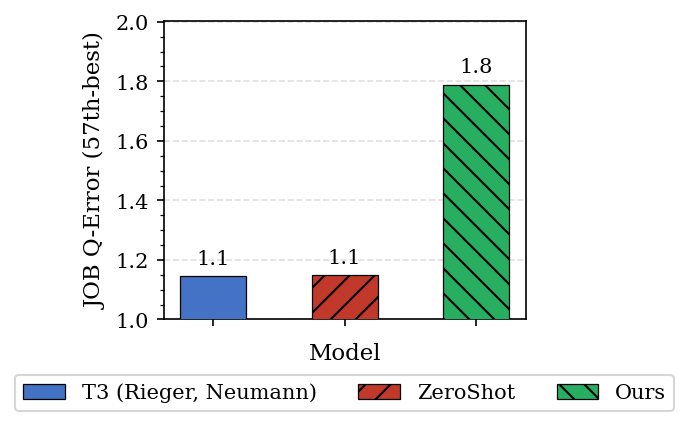
\includegraphics[width=0.7\textwidth]{figures/57th_comparison.png}
  \caption[57th-Best Q-Error Comparison]{57th-best Q-Error on the Join Order Benchmark for T3 (Umbra), ZeroShot, and our model.
  Values for T3 (Umbra) and ZeroShot are taken from Rieger \& Neumann ~\parencite{t3}}\label{fig:57th_comparison}
\end{figure}

\begin{figure}[htpb]
  \centering
  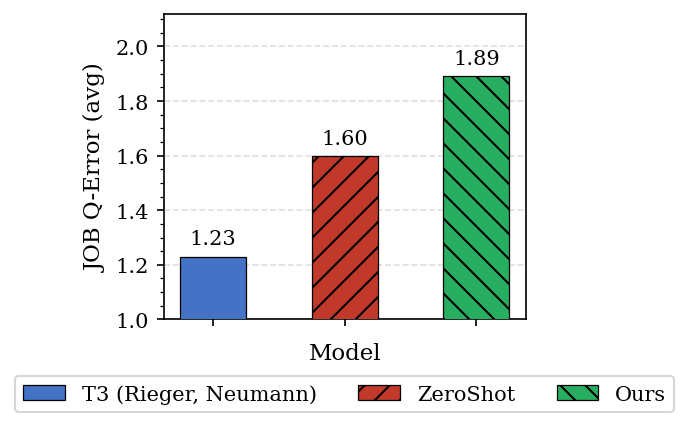
\includegraphics[width=0.7\textwidth]{figures/avg_comparison.png}
  \caption[Average Q-Error Comparison]{Average Q-Error on the Join Order Benchmark for T3 (Umbra), ZeroShot, and our model.
  Values for T3 (Umbra) and ZeroShot are taken from Rieger \& Neumann~\parencite{t3}.
  Our model's average is calculated over 77 instead of 113 queries.}\label{fig:avg_comparison}
\end{figure}

\paragraph{T3-based Models with Different Feature Vectors.}

Wehrstein et al. ran the JOB-Benchmark on their T3-based model and reported a median Q-Error of 4.07, using estimated cardinalities~\parencite{jobcomplex}.
Like before, they had the full 113 queries at disposal. We again use the 57th-best (p75) Q-Error value for the comparison with our model, this time selecting cardinality estimates.

Although we are in the worst-case-scenario, our model clearly outperforms Wehrstein et al.'s model, as Figure~\ref{fig:comp_wehrstein} shows.
A key difference between the models is the used feature vector, where only our model uses a completely PostgreSQL-native feature vector.
Hence, we demonstrate the relevance of PostgreSQL-native features.


\begin{figure}[htpb]
  \centering
  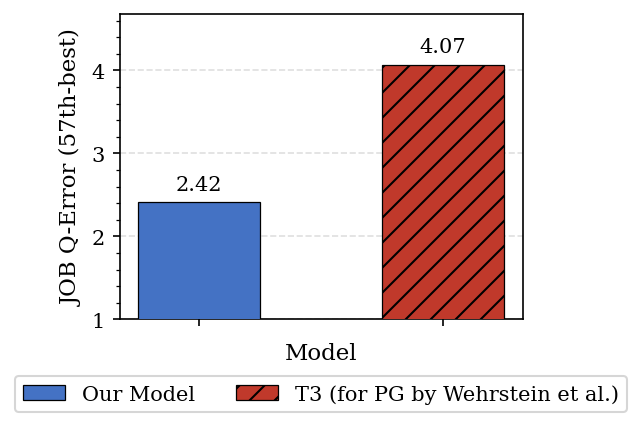
\includegraphics[width=0.7\textwidth]{figures/plot_comp_wehrstein.png}
  \caption[57th-Best Q-Error: Our Implementation vs.\ T3 for PostgreSQL]{57th-best Q-Error on the Join Order Benchmark. Our model against T3 adapted for PostgreSQL by Wehrstein et al~\parencite{jobcomplex}. Estimated cardinalities. }\label{fig:comp_wehrstein}
\end{figure}



\paragraph{Further PostgreSQL Prediction Models.}

Table~\ref{tab:median_qerror_job} shows the median Q-Error values for different learned cost models on the JOB-Benchmark using PostgreSQL and estimated cardinalities.
Once again, we use the 57th-best (p75) Q-Error value for the comparison with our model.

Here, the best performing models are neural networks like ZeroShot ~\parencite{zeroshot} and DACE ~\parencite{dace}, having a median Q-Error below 2.
Our model is in the top 4, coming in at 2.42, even when using a worst-case-scenario.
The remaining models are neural network-based estimators, such as QPPNet~\parencite{qppnet}.
They show a significant accuracy gap to the top performers, with median Q-Errors ranging from 8 to 18.
Finally, PostgreSQL's untrained, built-in cost estimator performs worst by a very large margin at a median Q-Error of over 1000, confirming the need for learned approaches.
Regarding learned approaches, not only neural networks can perform, but also decision trees like T3 for PostgreSQL.


\begin{table}[htpb]
  \centering
  \begin{tabular}{lc}
    \toprule
    \textbf{Model} & \textbf{Median Q-Error} \\
    \midrule
    Postgres (v16)  & 1015.67 \\
    DACE            & 1.91    \\
    E2E             & 13.21   \\
    FlatVector      & 2.15    \\
    MSCN            & 13.85   \\
    NEO             & 13.20   \\
    QPPNet          & 17.50   \\
    QueryFormer     & 8.30    \\
    ZeroShot        & \textbf{1.58}    \\
    Our model & 2.42 \\
    \bottomrule
  \end{tabular}
  \caption[Median Q-Error on JOB]{Median Q-Error on the Join Order Benchmark (JOB) across different models, data from Wehrstein et al.~\parencite{jobcomplex}. Our model reports the 57th-best (p75) Q-Error value, matching the median of the other models. Estimated cardinalities. }\label{tab:median_qerror_job}
\end{table}

\section{Ablation Study}\label{sec:evaluation_ablation}
\subsection{PostgreSQL-native Features vs. Direct Transfer}\label{subsec:eval_pg_vs_umbra_features}
\subsection{Actual vs. Estimated Cardinalities}

\subsection{Pipeline vs Tuple targets}


\section{Section}
Citation test~\parencite{latex}.

Acronyms must be added in \texttt{main.tex} and are referenced using macros. The first occurrence is automatically replaced with the long version of the acronym, while all subsequent usages use the abbreviation.

E.g. \texttt{\textbackslash ac\{TUM\}, \textbackslash ac\{TUM\}} $\Rightarrow$ \ac{TUM}, \ac{TUM}

For more details, see the documentation of the \texttt{acronym} package\footnote{\url{https://ctan.org/pkg/acronym}}.
\subsection{Subsection}

See~\autoref{tab:sample}, \autoref{fig:sample-drawing}, \autoref{fig:sample-plot}, \autoref{fig:sample-listing}.

\begin{table}[htpb]
  \caption[Example table]{An example for a simple table.}\label{tab:sample}
  \centering
  \begin{tabular}{l l l l}
    \toprule
      A & B & C & D \\
    \midrule
      1 & 2 & 1 & 2 \\
      2 & 3 & 2 & 3 \\
    \bottomrule
  \end{tabular}
\end{table}

\begin{figure}[htpb]
  \centering
  % This should probably go into a file in figures/
  \begin{tikzpicture}[node distance=3cm]
    \node (R0) {$R_1$};
    \node (R1) [right of=R0] {$R_2$};
    \node (R2) [below of=R1] {$R_4$};
    \node (R3) [below of=R0] {$R_3$};
    \node (R4) [right of=R1] {$R_5$};

    \path[every node]
      (R0) edge (R1)
      (R0) edge (R3)
      (R3) edge (R2)
      (R2) edge (R1)
      (R1) edge (R4);
  \end{tikzpicture}
  \caption[Example drawing]{An example for a simple drawing.}\label{fig:sample-drawing}
\end{figure}

\begin{figure}[htpb]
  \centering

  \pgfplotstableset{col sep=&, row sep=\\}
  % This should probably go into a file in data/
  \pgfplotstableread{
    a & b    \\
    1 & 1000 \\
    2 & 1500 \\
    3 & 1600 \\
  }\exampleA
  \pgfplotstableread{
    a & b    \\
    1 & 1200 \\
    2 & 800 \\
    3 & 1400 \\
  }\exampleB
  % This should probably go into a file in figures/
  \begin{tikzpicture}
    \begin{axis}[
        ymin=0,
        legend style={legend pos=south east},
        grid,
        thick,
        ylabel=Y,
        xlabel=X
      ]
      \addplot table[x=a, y=b]{\exampleA};
      \addlegendentry{Example A}
      \addplot table[x=a, y=b]{\exampleB};
      \addlegendentry{Example B}
    \end{axis}
  \end{tikzpicture}
  \caption[Example plot]{An example for a simple plot.}\label{fig:sample-plot}
\end{figure}

\begin{figure}[htpb]
  \centering
  \begin{tabular}{c}
  \begin{lstlisting}[language=SQL]
    SELECT * FROM tbl WHERE tbl.str = "str"
  \end{lstlisting}
  \end{tabular}
  \caption[Example listing]{An example for a source code listing.}\label{fig:sample-listing}
\end{figure}
